\chapter{Diseño y arquitectura del sistema}

\section{Estructura general}

El código del trabajo y todo lo que abarca se encuentra almacenando en \href{https://github.com/orgs/vieites-tfg/repositories?type=source}{GitHub}. Se han creado los repositorios necesarios en una misma organización de GitHub.

Entre los repositorios creados se pueden encontrar:

\begin{itemize}
  \item \texttt{zoo}.

    Este es el repositorio principal. Se trata de un \textit{monorepo}, en el que se encuentra implementado todo el código necesario dentro del presente trabajo de investigación. Dentro del repositorio se encuentran:
    \begin{itemize}
      \item La aplicación de prueba sobre la que se apoya el proyecto, y que da nombre al repositorio, debido a que se trata de una aplicación de gestión de un zoo.
      \item Los módulos de Dagger para realizar los ciclos de CI y CD.
      \item Otros archivos, como \textit{scripts} y archivos de configuración.
    \end{itemize}

  \item \texttt{helm-repository}.

    Este repositorio alberga las Charts de Helm que definen la estructura necesaria para desplegar la aplicación de prueba.

  \item \texttt{state}.

    Se trata del repositorio que, siguiento el enfoque GitOps, almacena los valores que poblarán los recursos de Kubernetes según el entorno en el que se despliegue la aplicación. Además, en este repositorio también existe una rama de despliegue, de la cual ArgoCD lee los manifiestos de los recursos que debe desplegar para cada uno de los entornos.
\end{itemize}

En la figura~\ref{fig:ghorg} se muestra un diagrama de la disposición de los repositorios y la relación entre ellos.

\section{zoo}

Como se ha comentado anteriormente, el repositorio \texttt{zoo} está estructurado como un \textit{monorepo}. Un \textit{monorepo} es un repositorio con diferentes proyectos, los cuales se encuentran interrelacionados de una manera bien definida. A lo largo de esta sección se justifica la elección de este tipo de estructura, a la vez que se explica cómo están implementados las diferentes piezas de software.

\subsection*{Aplicación de prueba}

La primera razón para escoger este tipo de estructura es el hecho de querer crear una aplicación relativamente pequeña, una página web que consta de un \textit{frontend} y un \textit{backend} (se hará referencia a estos como ``paquetes'' a partir de ahora). Por lo tanto, se hace más sencillo gestionar estos dos paquetes si se ubican en un único repositorio.

Otra ventaja de utilizar un \textit{monorepo} tiene que ver con el software utilizado para crear los paquetes de la aplicación de prueba. Ambos se implementan utilizando Node.js, en lenguaje Typescript\cite{ts}. Los paquetes tienen dependencias propias, y se puede dar el caso de que ambos utilicen una o varias dependencias iguales. Usar un \textit{monorepo} permite tener esas dependencias en un mismo lugar, evitando su duplicado. Con esto se consigue reducir el tiempo de construcción de los paquetes.

Sin embargo, es necesaria una herramienta que permita manejar los paquetes de manera independiente. Alguno de los motivos para tener esta preferencia pueden ser: que haya dos equipos de desarrolladores, uno para cada paquete; o que se quiera publicar versiones, hacer tests, u otro tipo de tarea sobre cada paquete por separado. La herramienta que se utiliza en este trabajo se llama Lerna\cite{lerna}. Este software está específicamente diseñado para gestionar \textit{monorepos} de proyectos de Node.js. Entre las ventajas que proporciona se encuentran:

\begin{itemize}
  \item Gestión de tareas locales.
  \item Cacheo local de salidas de comandos, con posibilidad de que dicha caché sea compartida entre entornos, por ejemplo, con agentes de CI.
  \item Detección de paquetes afectados por cambios en el código.
  \item Análisis de la estructura del proyecto.
\end{itemize}

Por los beneficios anteriormente comentados, y más, es por lo que se ha elegido esta herramienta para gestionar el \textit{monorepo}.

En cuanto a las tecnologías que se utilizan en la aplicación, ya se ha mencionado Typescript como lenguaje principal. Este lenguaje permite tener un sistema tipado, lo cual puede ser útil para detectar muchos errores comunes mediante el análisis estático en tiempo de construcción. Esto reduce las posibilidades de errores en tiempo de ejecución.

El \textit{backend} está completamente desarrollado utilizando dicho lenguaje. Su funcionalidad es proporcionar una API REST que el \textit{frontend} pueda utilizar para realizar cambios en la base de datos. Se usa MongoDB\cite{mongodb} como base de datos debido a que es fácil de gestionar y porque solo se almacena información sobre animales, sin ningún tipo de relación entre ellos, en una única tabla o documento.

El \textit{frontend} se ha implementado utilizando Vue.js\cite{vue}, un \textit{framework} que permite construir interfaces web mediante componentes reactivos. Se ha escogido este frente a otras opciones debido a su facilidad de uso sin conocimiento previo. Tiene una API intuitiva, por lo que no tiene una gran curva de apendizaje. Además, el propio \textit{framework} está construido utilizando Typescript, por lo que tiene compatibilidad de primera clase con este lenguaje.

En la figura \ref{fig:app} se puede ver un diagrama que muestra cómo es la comunicación entre los paquetes de la aplicación, y con la base de datos, junto con las tecnologías que se utiliza en cada uno de ellos.

\begin{figure}
  \centerline{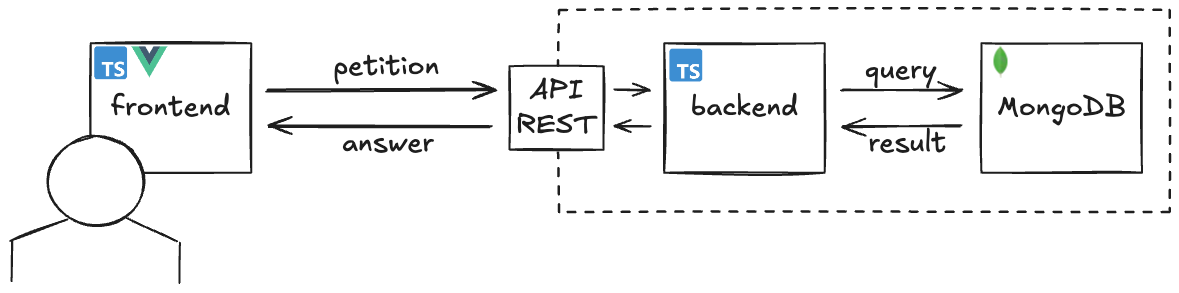
\includegraphics[width=15cm]{figuras/app}}
  \caption{Comunicación entre paquetes de la aplicación. Imagen creada con \href{https://excalidraw.com}{excalidraw.com}}
  \label{fig:app}
\end{figure}

\subsection*{Módulos de Dagger}

Se integran también en el repositorio los módulos de Dagger de CI y de CD. Estos módulos se incluyen en el \textit{monorepo} para facilitar la referencia a los paquetes que constituyen la aplicación de prueba. Además, resulta lógico que se ubiquen en el mismo lugar una aplicación y las herramientas que permiten su evolución, como son cualquier tipo de \textit{software} que realice las funciones de CI y de CD.

Ambos módulos se realizan utilizando el SDK del lenguaje Go que proporciona Dagger. Se ha escogido este lenguaje debido al conocimiento previo que ya se tenía de este. Además, es el lenguaje en el que está implementado el propio Dagger.

Uno de los módulos se encarga del ciclo de CI, es decir, de realizar los tests de la aplicación, del \textit{linting} o análisis del código en sí, y de la publicación de imágenes de Docker y paquetes NPM. Está organizado de manera que se pueden gestionar cada uno de los paquetes de la aplicación de manera independiente. Esto también es posible gracias al uso de Lerna, que ya se ha comentado anteriormente.

El segundo de los módulos, el de CD, realiza la tarea de publicación de los recursos de Kubernetes, los cuales son posteriormente obtenidos por ArgoCD para su despliegue completo. Esto se consigue haciendo uso de los repositorios \texttt{helm-repository} y \texttt{state}, en los cuales se almacenan las Charts de Helm y los valores que pueblan dichas Charts, respectivamente.

Se detalla más profundamente la implementación de los módulos de Dagger en el capítulo \ref{chap:dagger}.

\subsection*{Creación y configuración de los \textit{clusters}}
\label{subsec:clusters}

La fase final del ciclo de una aplicación es el despliegue. En este trabajo se levantan tres \textit{clusters} de KinD de manera local. Estos son los lugares en los que se despliega la aplicación. Generalmente se tienen diferentes \textit{clusters} con el fin de probar la aplicación en entornos distintos antes de desplegarla en el principal, que sería el de producción. El hecho de crearlos todos localmente hace que sean más sencillas las pruebas relacionadas con el despliegue. En equipos de desarrollo reales, los entornos de producción se encuentran en la nube. Sin embargo, sí que se pueden llegar a tener entornos locales para realizar pruebas de la aplicación.

Los \textit{clusters} se crean con el \textit{script} que se muestra en el Listing \ref{lst:create-clusters} (se han puesto comentarios en vez de código algunas partes para reducir su tamaño, a modo de pseudocódigo). Este \textit{script} está escrito para funcionar en sistemas UNIX, en Bash, por lo que es un requisito utilizar un sistema operativo como MacOS o una distribución de Linux para probar el \textit{script}. No funcionará en un sistema operativo Windows. A modo de resumen del \textit{script}:

\begin{itemize}
  \item Se crean tres \textit{clusters} con su configuración específica. Se puede ver el archivo de configuración del \textit{cluster} de \texttt{dev} en el Listing \ref{lst:conf-cluster}.
  \item Se instala en cada \textit{cluster} un controlador de Ingress, lo cual permitirá acceder a la aplicación a través de una URL customizada desde el exterior.
  \item Se incluye como Secret el valor de la clave de cifrado que permite desencriptar los secretos. El proceso de creación de cifrado y descifrado se explica en \ref{subsec:secretos}.
  \item Se instala la Chart de Helm de Argo. A esta Chart se le pasan una serie de valores, de los cuales se habla en \ref{subsec:secretos}. Más información sobre cómo acceder a la interfaz de Argo en
    \begin{bclogo}[logo=\bcattention]{Important!}
      CITAR MANUAL DE USUARIO
    \end{bclogo}
  \item Se aplica la configuración específica de Argo para el entorno que se está creando. Se puede ver la configuración para Argo en el entorno de \texttt{dev} en el Listing \ref{lst:conf-argo}. En dicha configuración se indica el repositorio, la ruta desde la raíz donde se encuentran los recursos y la rama de donde Argo debe obtener los archivos que definen los recursos que se van a desplegar.
  \item Se añade un banner en la parte superior de la interfaz para distinguir cada uno de los \textit{clusters}.
  \item Se muestra la contraseña del usuario \texttt{admin}, para poder hacer \textit{log in} a través de la interfaz de Argo.
\end{itemize}

En la figura \ref{fig:clusters} se puede observar cómo se sincroniza ArgoCD, en cada uno de los \textit{clusters}, con el repositorio de estado. Argo reacciona cada vez que se realizan cambios en el directorio que le corresponde, dentro de la rama de despliegue del repositorio \texttt{state}. En ese momento, obtiene de nuevo todos los archivos de definición de los recursos y se sincroniza con el estado deseado.

\subsection*{Gestión de secretos}
\label{subsec:secretos}

La aplicación de prueba consta de una base de datos, la cual tiene usuario y contraseña. Este es un ejemplo de datos que es necesario almacenar como un secreto o Secret de Kubernetes. Debido a que se está utilizando un método \textit{pull}\cite{pull} de despliegue de la aplicación; es decir, la herramienta que realiza el despliegue, ArgoCD, ``tira'' (hace \textit{pull}) del repositorio que le indicamos como objetivo; es necesario almacenar en el repositorio los secretos encriptados previamente. Esto es una buena práctica para evitar que se filtren sin querer los datos al exterior, aunque el repositorio sea privado.

Existe un apartado completamente dedicado a como se realiza la gestión de secretos en \ref{sec:secrets}. 

\subsection*{Función de cada \textit{cluster} y promoción de entornos}
\label{subsec:cluster-func}

A continuación se explica para qué se utiliza cada \textit{cluster} y cuál es el proceso de despliegue de la aplicación en cada uno de los entornos.

\begin{itemize}
  \item \texttt{dev}.

    Se trata del \textit{cluster} de desarrollo. En este se despliega la aplicación en el momento en el que se añade una nueva funcionalidad, ya sea en el \textit{frontend} o en el \textit{backend}. Esto implica, en términos de GitHub:

    \begin{enumerate}
      \item Crear una \textit{Pull Request} (PR) en la que se implementa la nueva funcionalidad. Esta debe ser lo más reducida posible, cumpliendo con la filosofía de CI. Esto implica que la intención del equipo de desarrollo debe ser desplegar nuevas funcionalidades o correcciones de errores en producción en el menor tiempo posible. Se puede conseguir esto planeando PRs cortas en cuanto a tiempo de desarrollo, evitando que el equipo tenga demasiado trabajo en progreso y asignando los recursos necesarios para que cada PR se lleve a cabo lo más rápidamente\cite{linear}.
      \item Implementar la funcionalidad o realizar la corrección pertinente. A medida que se implementa, se puede, y es una buena práctica, ejecutar localmente el ciclo de CI para asegurarnos de que se pasan las pruebas y el \textit{linting} del código. Esta es una de las ventajas principales de utilizar Dagger. El desarrollador puede comprobar de manera local si el código actualizado es capaz de pasar el \textit{pipeline} de CI, lo cual evita tener errores inesperados a la hora de integrar el código en la rama principal.
      \item Revisar que la tarea que correspondía hacer en dicha PR se ha realizado correctamente.
      \item Integrar la funcionalidad o corrección en la rama principal del repositorio.
    \end{enumerate}

    Tras haber terminado todos los pasos anteriores, se ejecuta un \textit{workflow} de GitHub que realiza todo el ciclo de CI y CD, independientemente del entorno en el que se vaya a desplegar. El \textit{workflow} es el que se ve en el Listing \ref{lst:workflowcicd}. Para más información sobre los pasos que son necesarios pala la promoción de entornos ver \ref{sec:promotion}. 

    Lo que se consigue con el \textit{workflow} mencionado es ejecutar los \textit{pipelines} de CI y de CD para la versión actual de la aplicación, lo cual permite desplegarla completamente en el entorno que le corresponde. El entorno en el que se despliega depende del evento que produce la ejecución del \textit{workflow}, que puede ser: una integración de código en la rama principal, la creación de una \textit{prerelease} o la creación de una \textit{release}. Los eventos anteriores hacen que se despliegue en \texttt{dev}, \texttt{pre} y \texttt{pro}, respectivamente.

  \item \texttt{pre}

    Este es el entorno de pre-producción. Este tipo de entornos están diseñados para simular el entorno de producción real, y funciona como prueba final previa a la publicación de una aplicación. En el caso de este trabajo, como ya se ha comentado, todos los entornos son idénticos, pero en equipos y entornos reales, cada uno de ellos tiene características distintas.

  \item \texttt{pro}

    Finalmente, el entorno de producción. Aquí es donde se despliega la aplicación de manera abierta a los usuarios. Como se lleva insistiendo a lo largo de este capítulo, lo normal es que estos entornos se encuentren en la nube. Para mayor facilidad de pruebas y debido a que no es la finalidad de este trabajo, se ha decidido crear todos los \textit{clusters} de forma local.

\end{itemize}

En la figura \ref{fig:promotion} se muestra cómo el \textit{workflow} escucha los diferentes eventos que hacen que se ejecute el ciclo de CI/CD. Dependiendo del evento que ocurre, se va a utilizar una \textit{tag} diferente y se va a desplegar en el entorno correspondiente.

\section{helm-repository}
\label{subsec:helm}

Es una práctica habitual tener un repositorio con todas las Charts de Helm que utiliza el equipo de desarrollo. Esto permite tener un lugar centralizado para que los desarrolladores compartan y los usuarios encuentren aplicaciones para desplegar en Kubernetes.

Este repositorio tiene como finalidad lo que se acaba de comentar, funcionar como el lugar en el que se almacena la Chart de Helm de la aplicación de prueba.

La figura \ref{fig:helm-repository} muestra que se ha creado una Chart \textit{umbrella} llamada \texttt{zoo}. Una Chart de este tipo funciona como una agrupación de más \texttt{subcharts} que están interrelacionadas. Normalmente se utiliza este método para gestionar despliegues de aplicaciones complejas en Kubernetes.
La definición de la Chart \texttt{zoo} se puede ver en el Listing \ref{lst:umbrella}. En esta se indican las dependencias (\textit{subcharts}) que agrupa la Chart. Entre estas se encuentran las Charts propias de la aplicación, \texttt{zoo-frontend} y \texttt{zoo-backend}. Además, se puede ver que se utiliza una Chart ya definida en un repositorio conocido, perteneceinte a Bitnami\cite{bitnami}. De este repositorio se obtiene la Chart de MongoDB. De esta manera, se utiliza una Chart ya implementada y desarrollada por expertos, proporcionando muchas opciones de configuración y ofreciendo mucha más seguridad de lo que se tendría en el caso de crear una Chart de Mongo propia para la aplicación.

También se puede observar en la figura \ref{fig:helm-repository} los recursos que se crean para cada una de las \textit{subcharts} de la aplicación. Para más detalle en cuanto a su funcionamiento, ver \ref{tech:k8s}.

Se detalla el proceso de desarrollo de la Chart de la aplicación en \ref{sec:chart}.

\section{state}
\label{subsec:state}

El repositorio de estado funciona como única fuente de verdad. Aquí se definen  los valores que pueblan la Chart de la aplicación. Se utiliza una herramienta llamada \texttt{helmfile}\cite{helmfile}. Esta permite integrar Charts de Helm y valores, aunque estos se encuentren en lugares diferentes. En la figura \ref{fig:state} se muestra la estructura del repositorio de estado, incluyendo la rama principal y la rama de despliegue.

Se puede ver el archivo de configuración de \texttt{helmfile} en el Listing \ref{lst:helmfile}. Los archivos del apartado de \texttt{environments} indican el \textit{namespace} y la versión de la Chart que se va a utilizar. Todos los valores que se indican en el apartado de \texttt{releases} dependen del entorno que se ha elegido para desplegar. Los valores de las líneas 19-22 son aquellos que no dependen del entorno en el que se quiere desplegar, mientras que los de las líneas 23-26 sí que dependen del entorno, y se almacenan en un directorio dedicado a cada uno de ellos. En estos últimos archivos de valores dependientes del entorno se indica, por ejemplo, la \textit{tag} a utilizar de las imágenes de Docker.

Un ejemplo de archivo de valores se puede observar en el Listing \ref{lst:values}. Como se ha comentado, el valor de la \textit{tag} se ve indicado en la línea 3, con el formato que se menciona en \ref{sec:promotion}.

En la sección
\begin{bclogo}[logo=\bcattention]{Important!}
  CITAR SECCIÓN DE DAGGER CD
\end{bclogo}
se explica cómo se especifica el entorno y, por lo tanto, los valores que se van a utilizar para poblar la Chart de la aplicación.

Este repositorio también es el lugar en el que se almacenan los archivos que definen los recursos que se van a desplegar en cada entorno. En la figura \ref{fig:secrets} se puede ver la estructura que tiene uno de los directorios (\texttt{dev}) de la rama de despliegue del repositorio \textit{state}. La estructura de dicho directorio en la rama \texttt{deploy} es la misma para los directorios correspondientes a los demás entornos.
